\chapter{Results}
\label{chap:Results}

\section{Classification}
\label{sec:classification_results}


\begin{figure}[H]
    \center
    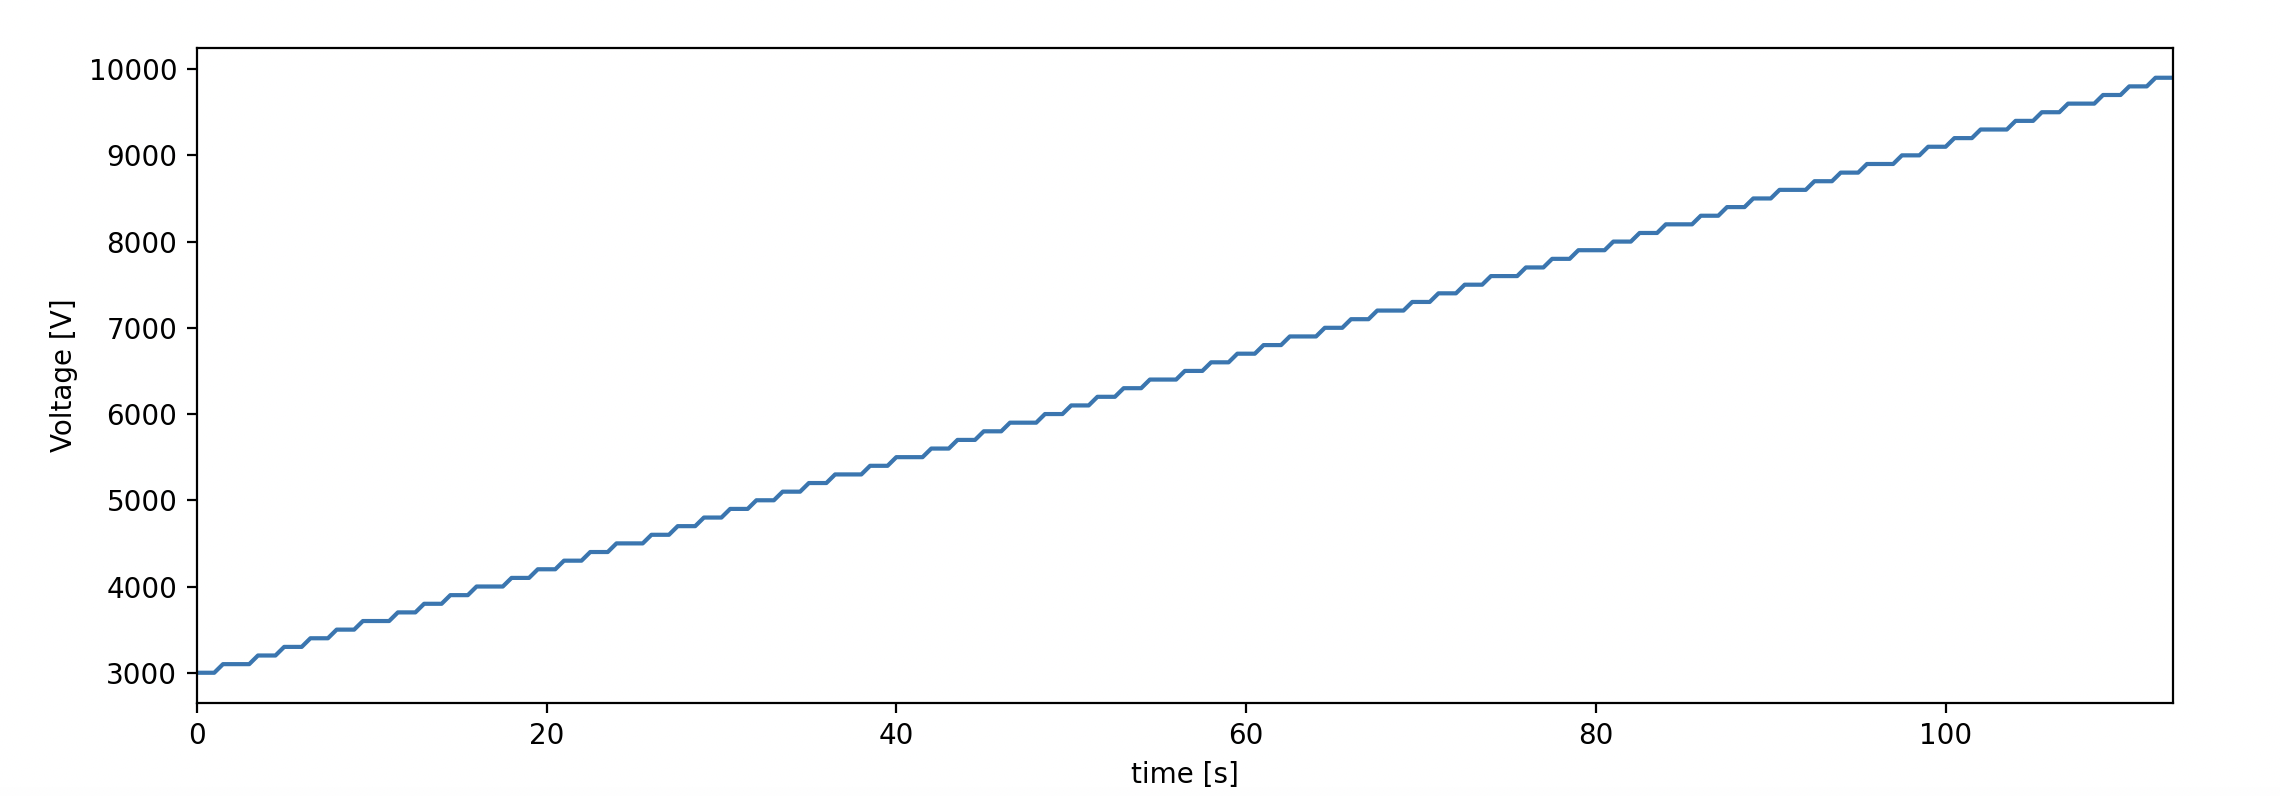
\includegraphics[width=12cm]{Figuras/19:03/voltage_step.png}
    \caption{ exp-26-01-2 (V x Q)}
\end{figure}


\begin{figure}[H]
    \center
    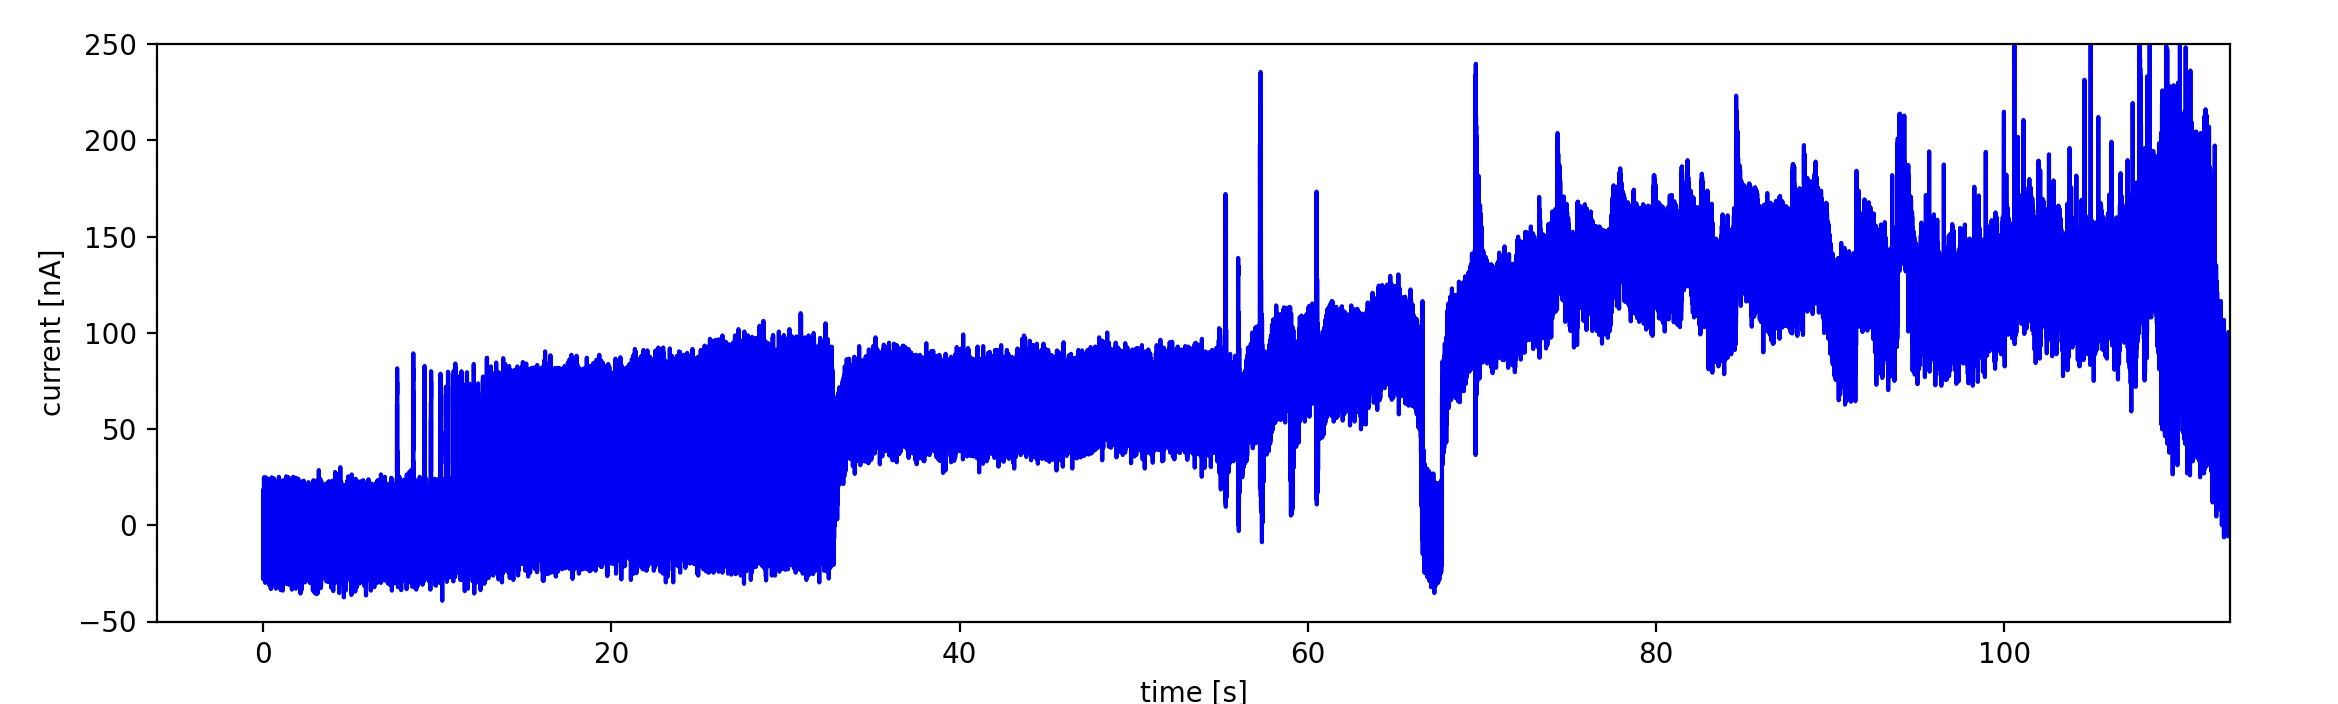
\includegraphics[width=12cm]{Figuras/19:03/raw-data-example.png}
    \caption{ exp-26-01-2 (V x Q)}
\end{figure}


\begin{figure}[H]
    \center
    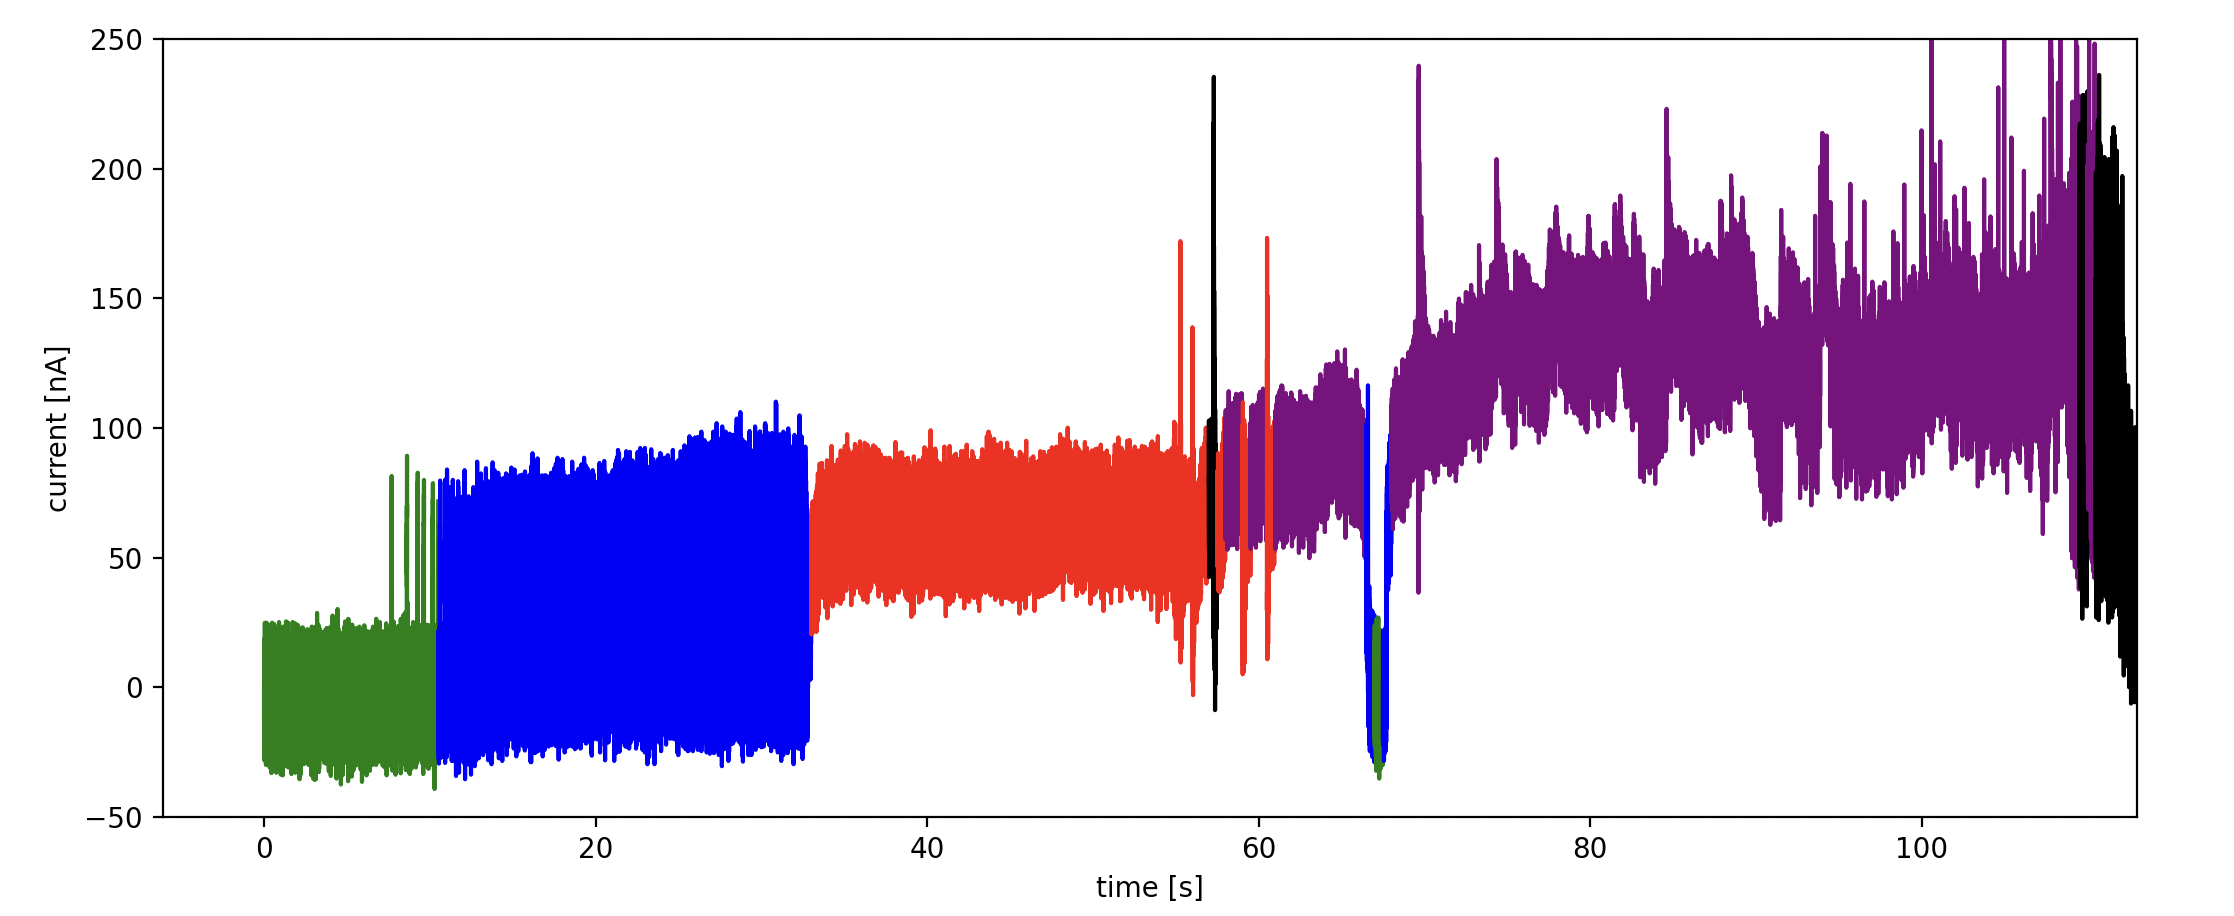
\includegraphics[width=12cm]{Figuras/19:03/classified-data-example.png}
    \caption{ exp-26-01-2 (V x Q)}
\end{figure}


\section{Map Sequence}
\label{sec:map_results}



\subsection{Manual experiments}


For better understand the effects of both voltage and flowrate in the spraying dinamycs manual experiments were made.
Also in order to find the stability region of cone jet mode for the liquid and setup used.



\begin{figure}[H]
    \center
    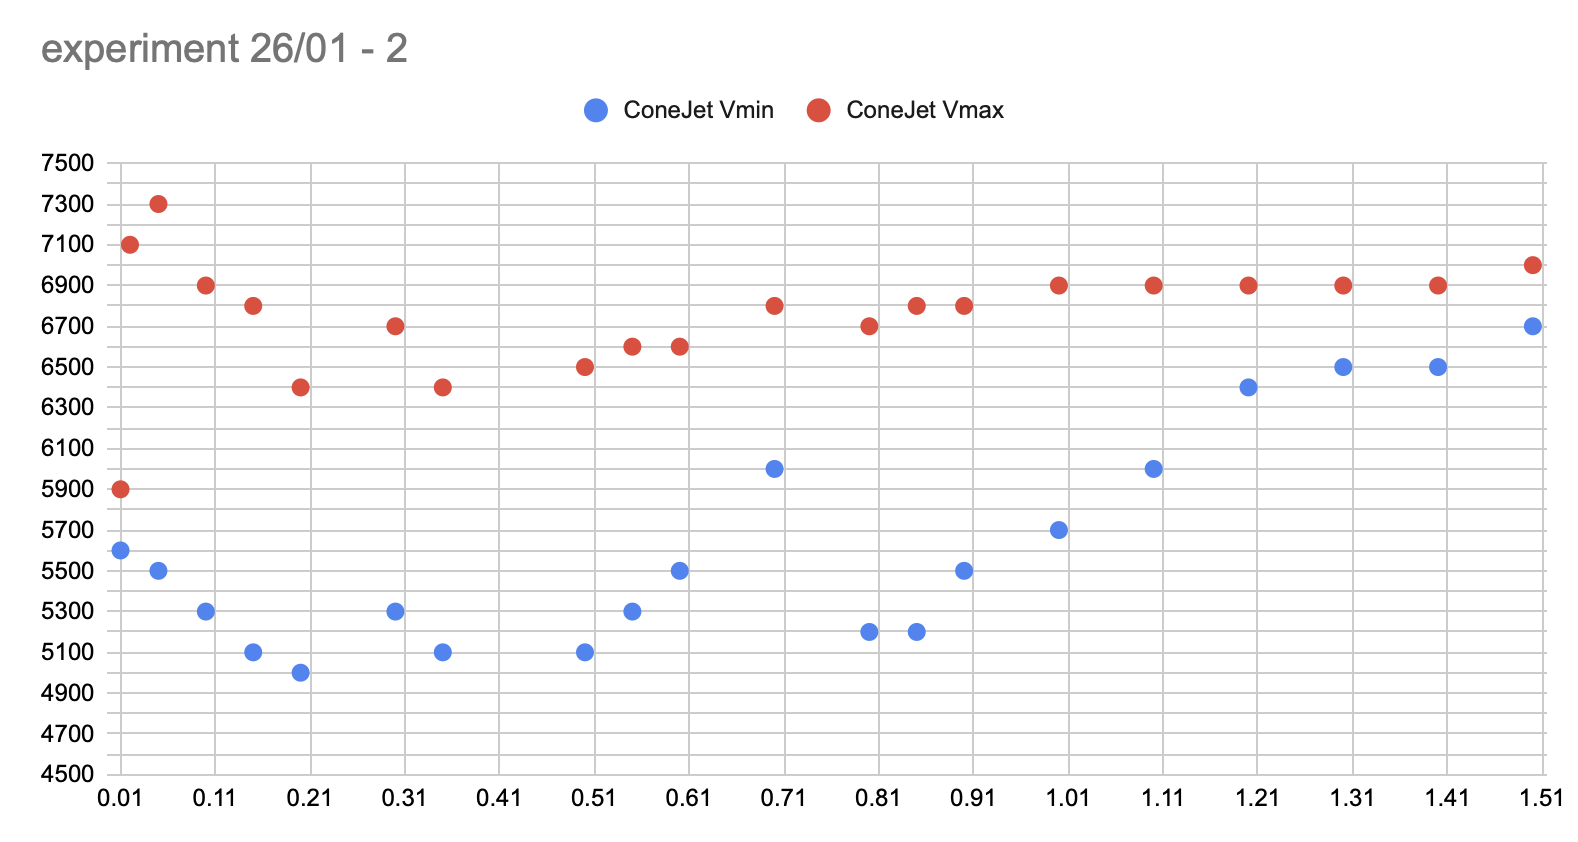
\includegraphics[width=12cm]{Figuras/report3/exp26-01-2.png}
    \caption{ exp-26-01-2 (V x Q)}
\end{figure}


\begin{figure}[H]
    \center
    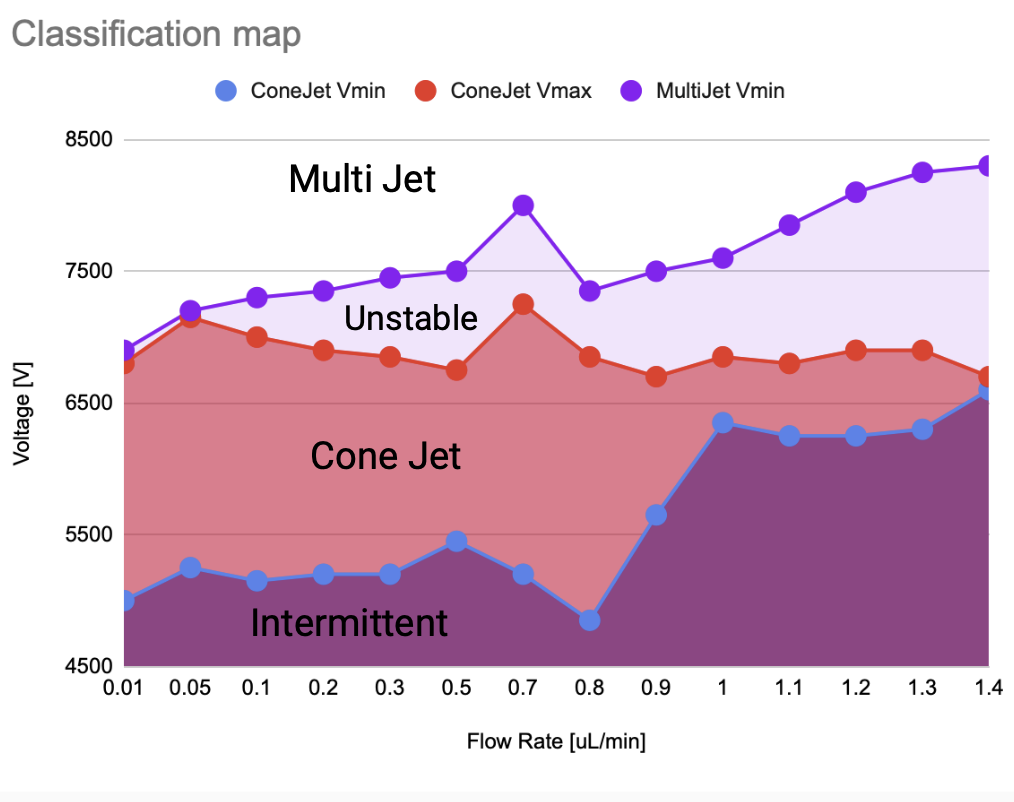
\includegraphics[width=12cm]{Figuras/regions.png}
    \caption{ exp-26-01-2 (V x Q)}
\end{figure}


\subsection{Automatic experiments}

With the desired voltage and flowrate range defined for the automatic experiment the next part is to define how many datapoints will be collected in both
x and y axis. Since we are introducing a new dimension for our experiment it is also increasing fast the amount of data collected.
The goal of this part is to find the ideal combination of voltage step size, voltage step time and flowrate step size in order to get the most accurate results without exceding the separate memory for each experiment.

In the further improvements of the routine it's ideal to apply a real time file writing with all experiment data.
This will prevent that any crashes in the program lose all data and not overflow the memory allocated for the program.


\begin{multicols}{3}


    \begin{figure}[H]
        \center
        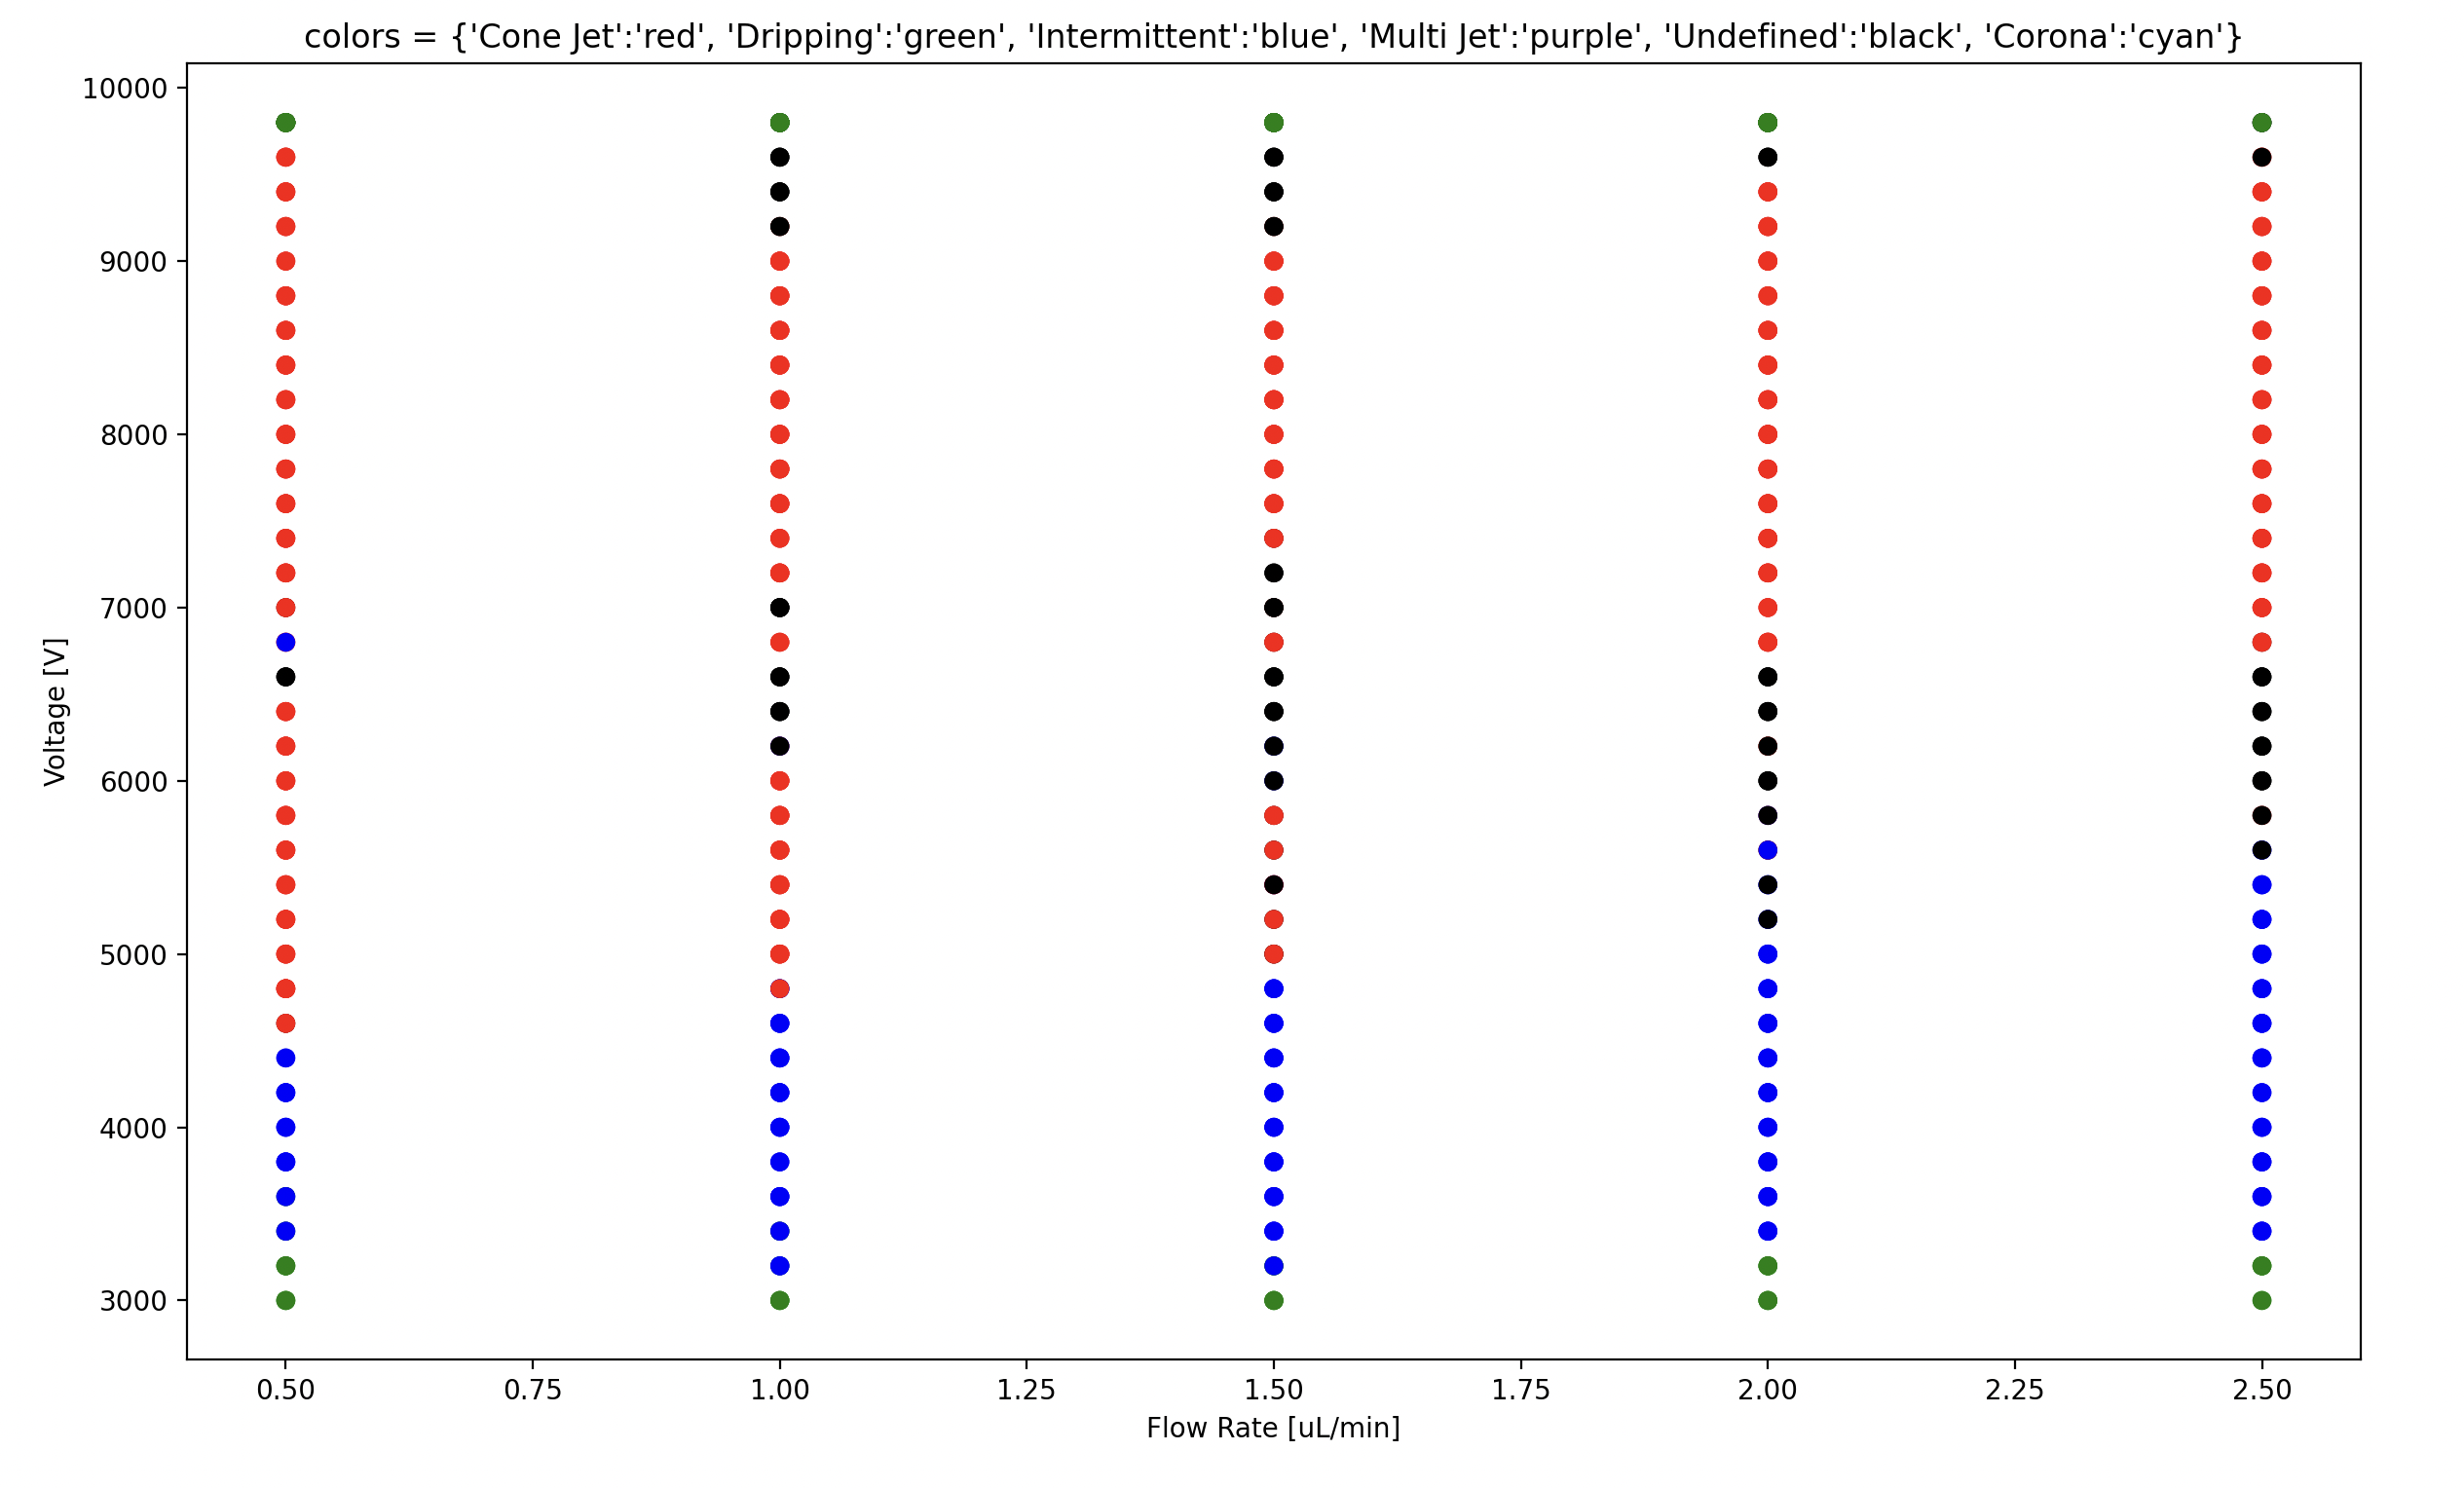
\includegraphics[width=5cm]{Figuras/report3/map1.png}
        \caption{First mapping trial}
    \end{figure}

    \begin{figure}[H]
        \center
        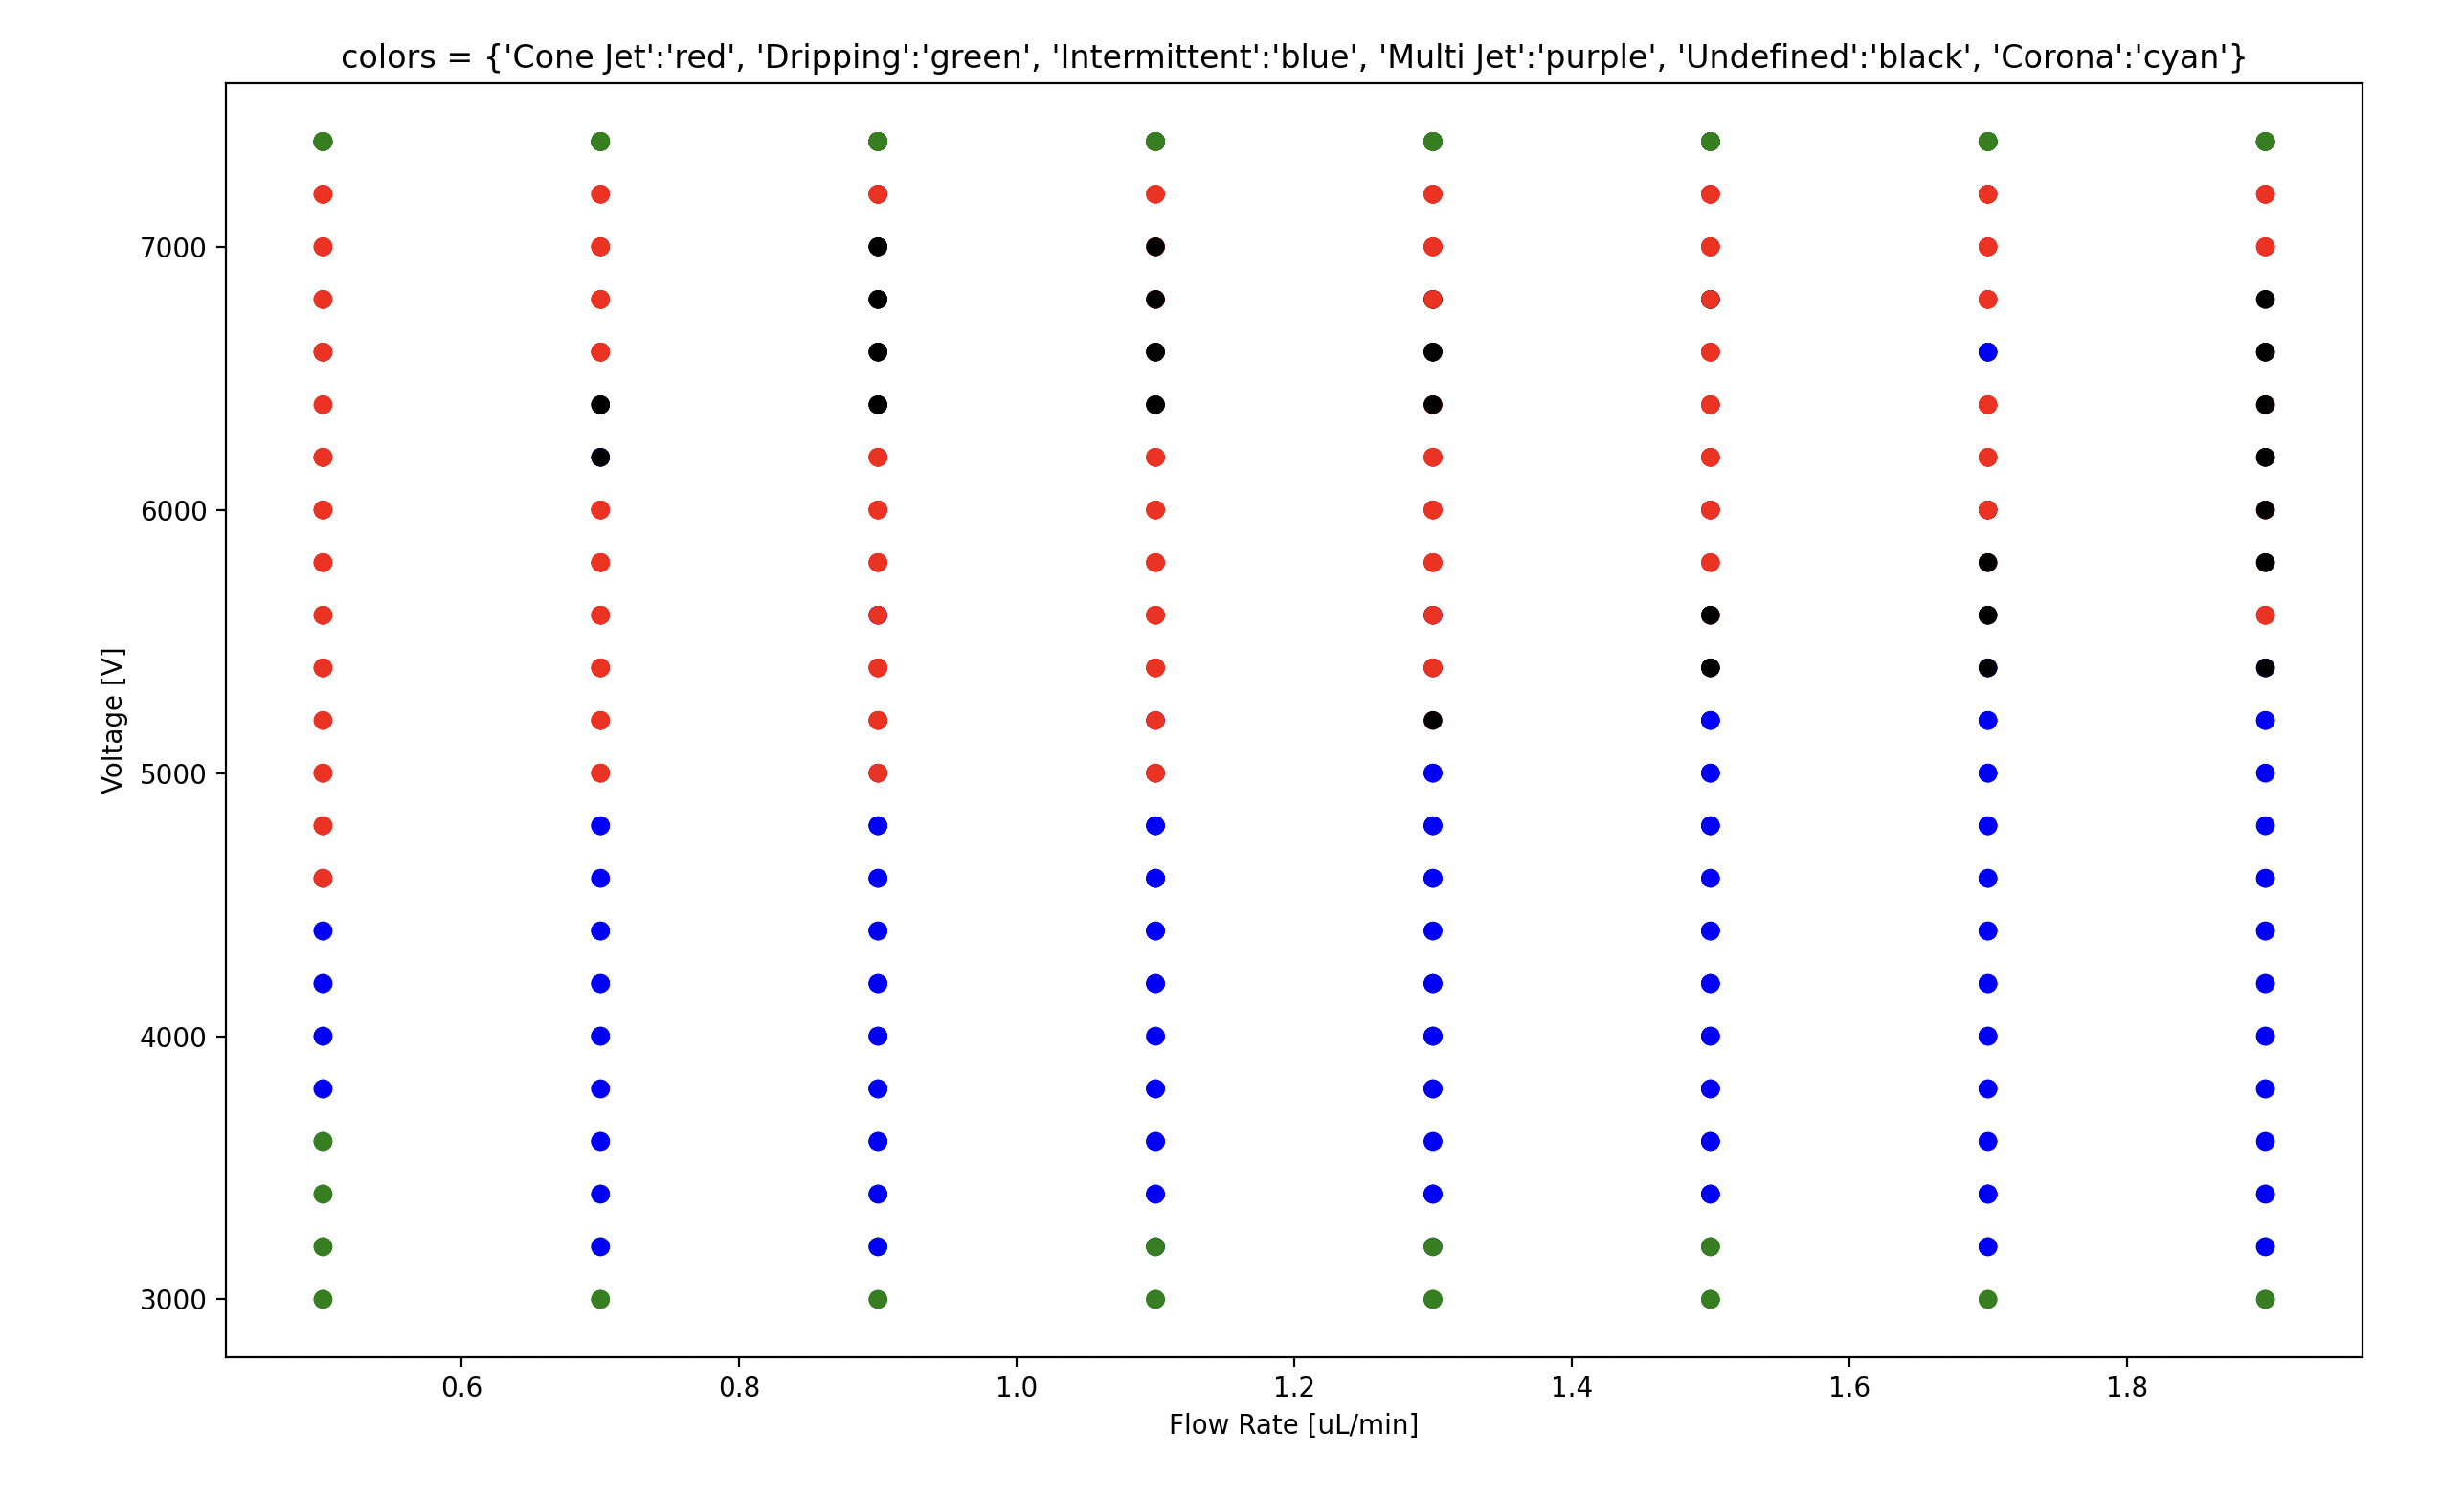
\includegraphics[width=5cm]{Figuras/report3/map2.png}
        \caption{Second mapping trial}
    \end{figure}


    \begin{figure}[H]
        \center
        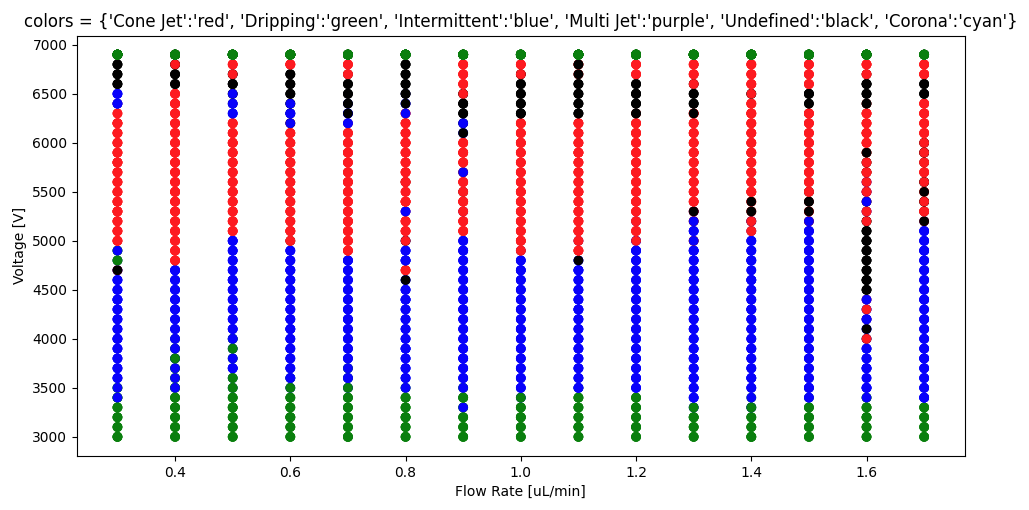
\includegraphics[width=6cm]{Figuras/report3/map3.png}
        \caption{third map - better result}
    \end{figure}

\end{multicols}



\subsection{Manual x Automatic Cone Jet stability island maps}

For validation of the automatic system and classification some experiments were made having both manual and automatic data collecting.

The Figure 13 shows a printscreen of how the experiment looks like in real time.
We can see the image generated by the camera in the back.
The routine code running in pycharm software on the right.
And also real time signal plottings of the current data on the left.

\begin{figure}[H]
    \center
    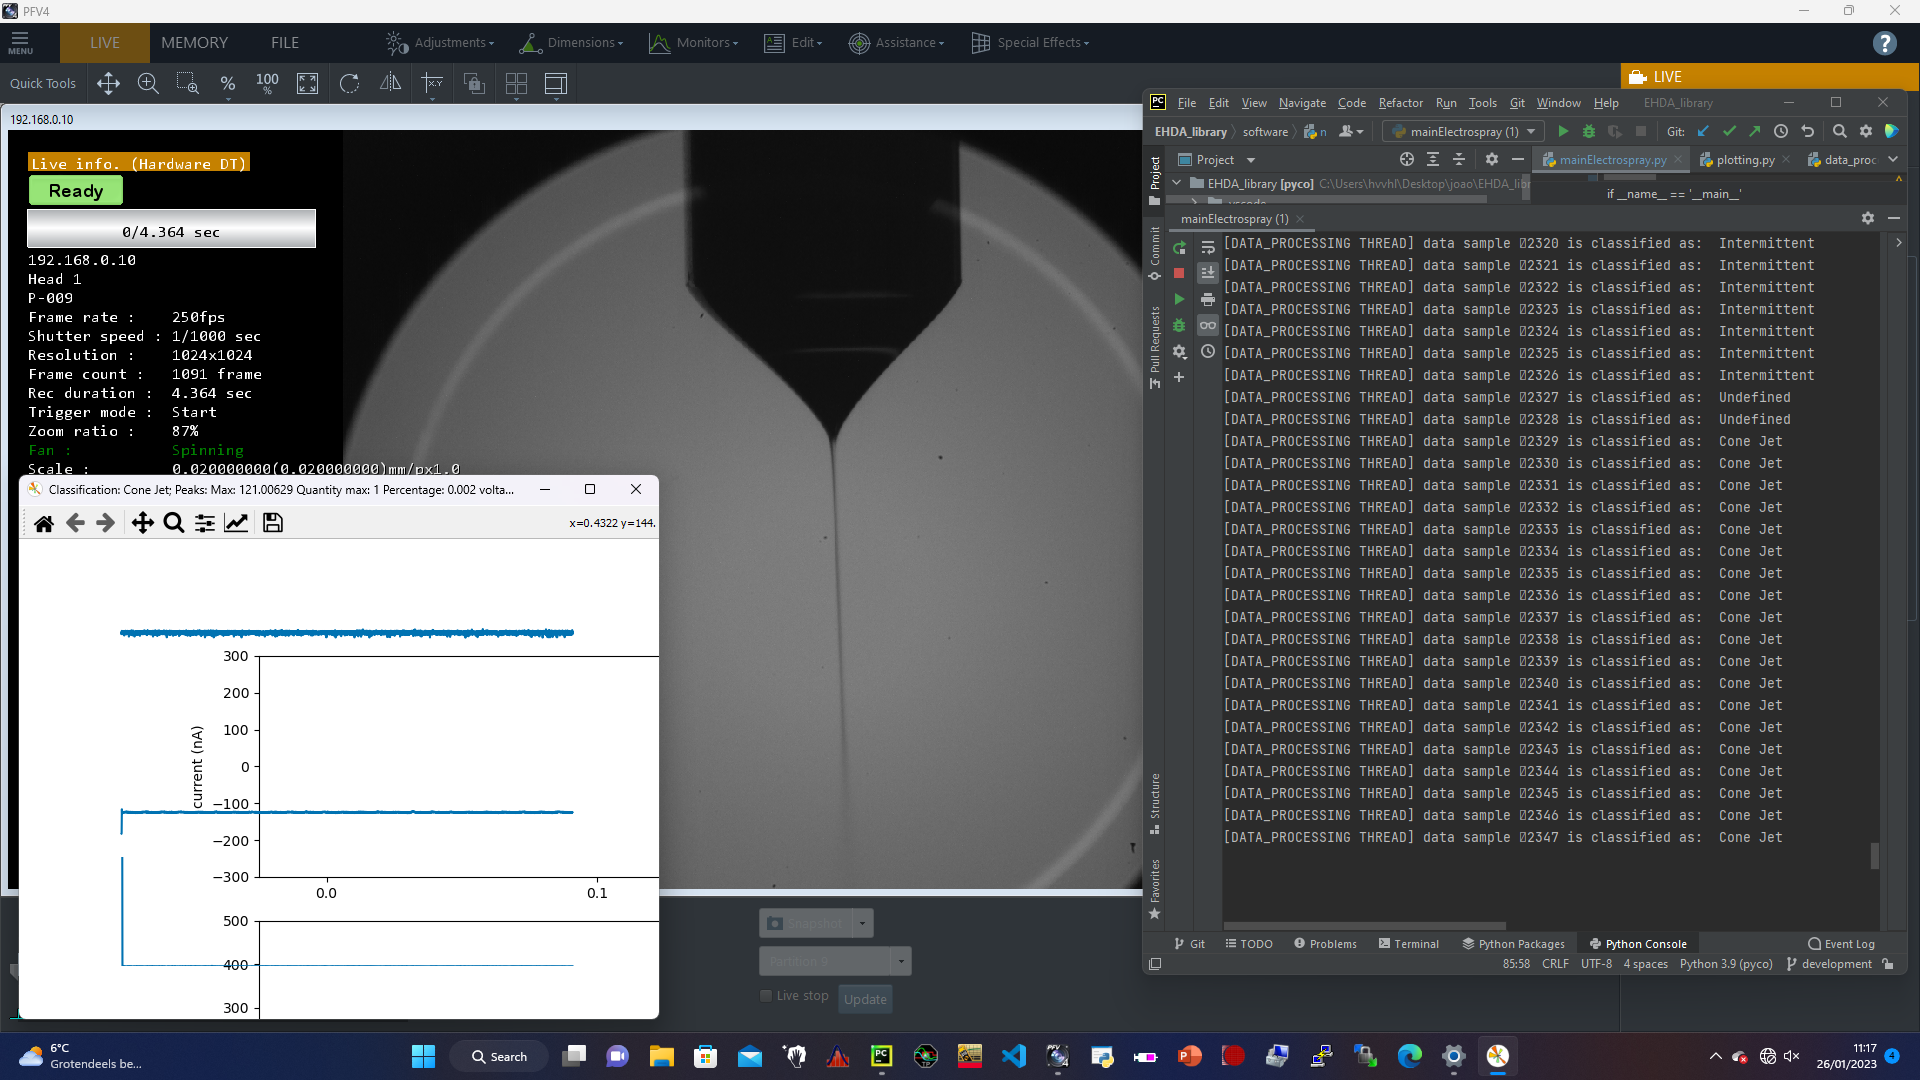
\includegraphics[width=17cm]{Figuras/report3/screenshots/stableConeExp.png}
    \caption{running experiment print screen}
\end{figure}

In Figure 14 we can see a result of the map generated by the automatic classification in this experiment.

\begin{figure}[H]
    \center
    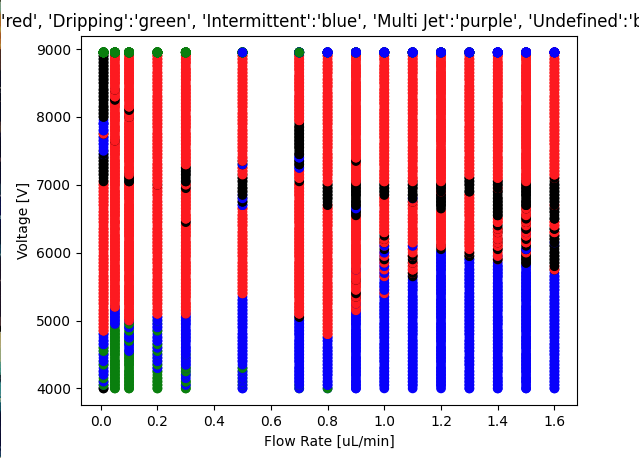
\includegraphics[width=10cm]{Figuras/report3/map-exp-26-01.png}
    \caption{ exp-26-01-23 }
\end{figure}

Figures 15 and 16 shows that we could achieve a stable cone jet region map with similar shape and values in both manual and automatic classification of the same experiment.

\begin{multicols}{2}


    \begin{figure}[H]
        \center
        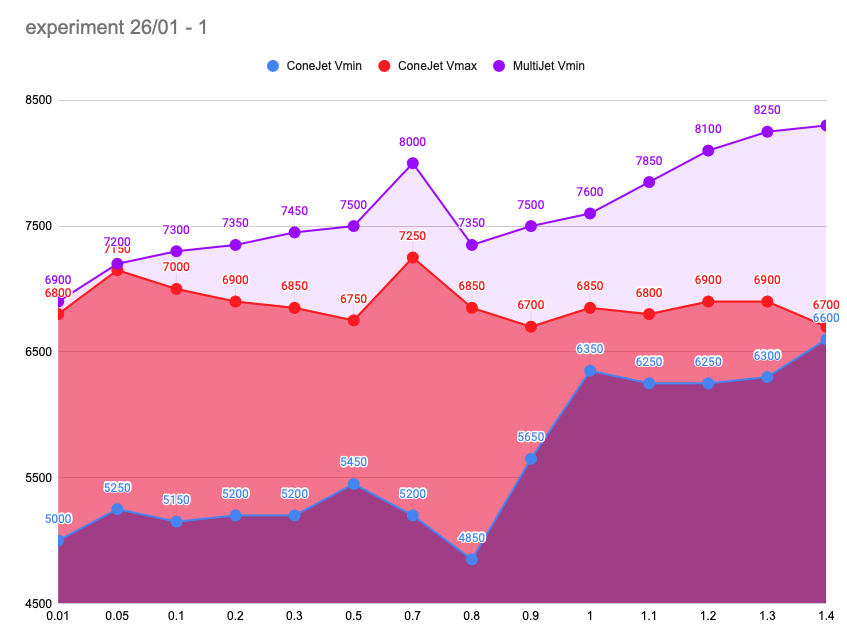
\includegraphics[width=9cm]{Figuras/report3/manual-mapping.png}
        \caption{ exp-26-01 manual classification}
    \end{figure}

    \begin{figure}[H]
        \center
        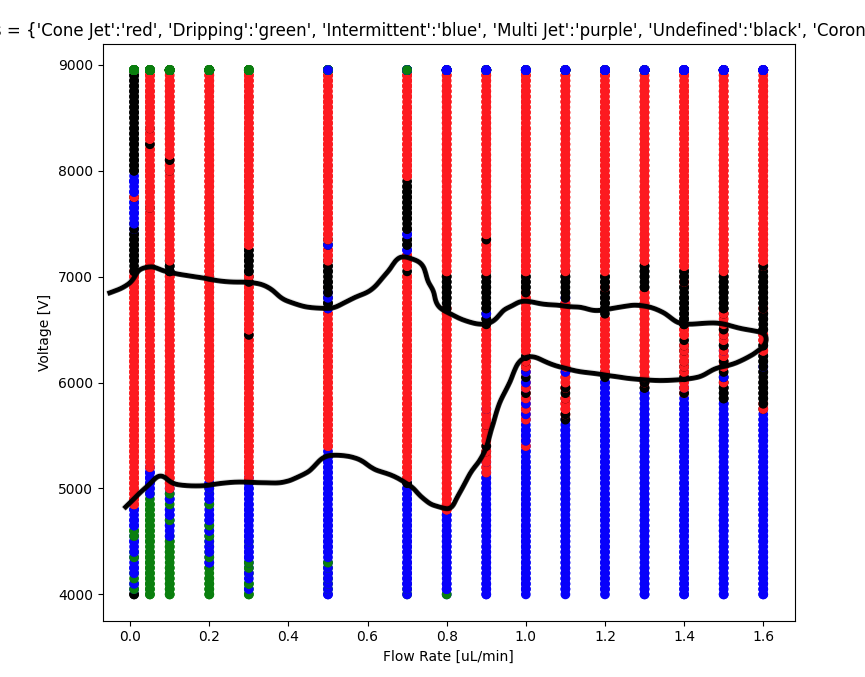
\includegraphics[width=9cm]{Figuras/report3/map4-stabilityIsland.png}
        \caption{ exp-26-01 automatic classification}
    \end{figure}

\end{multicols}

Figures 15 and 16 shows that we could achieve a stable cone jet region map with similar shape and values in both manual and automatic classification of the same experiment.

Figures 15 and 16 shows that we could achieve a stable cone jet region map with similar shape and values in both manual and automatic classification of the same experiment.


\begin{multicols}{2}


    \begin{figure}[H]
        \center
        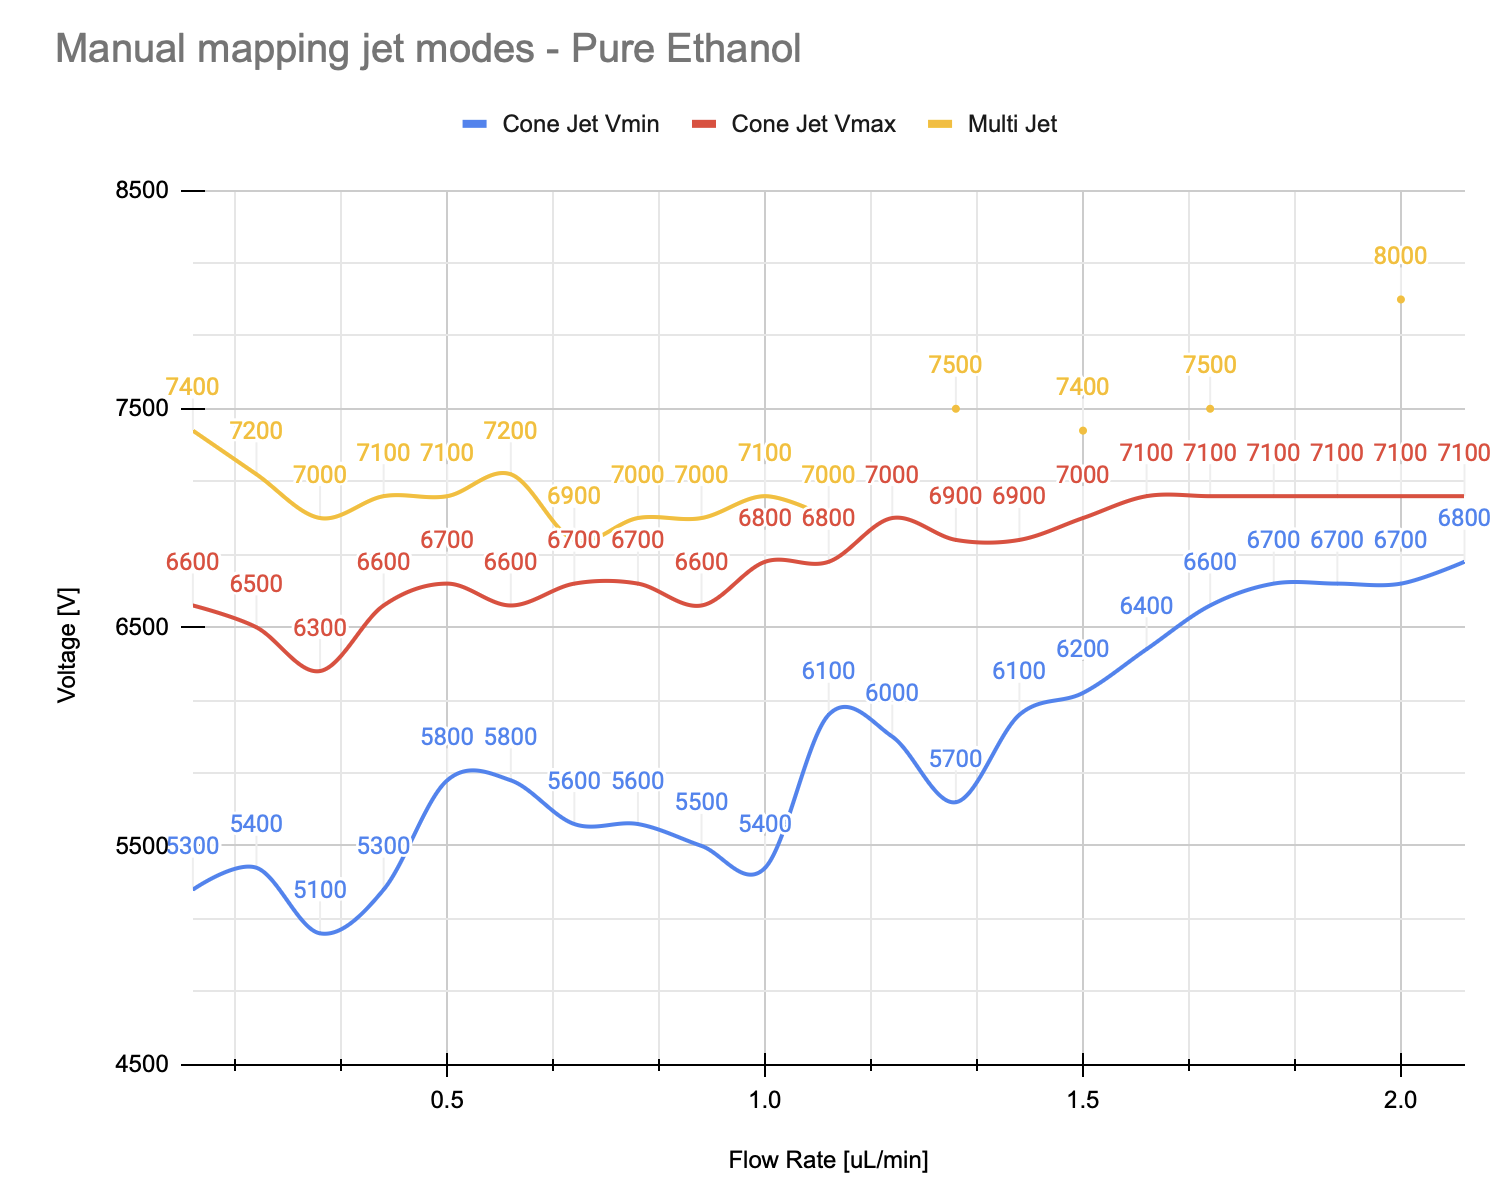
\includegraphics[width=7cm]{Figuras/report4/map7-manual.png}
        \caption{ exp-26-01 manual classification}
    \end{figure}

    \begin{figure}[H]
        \center
        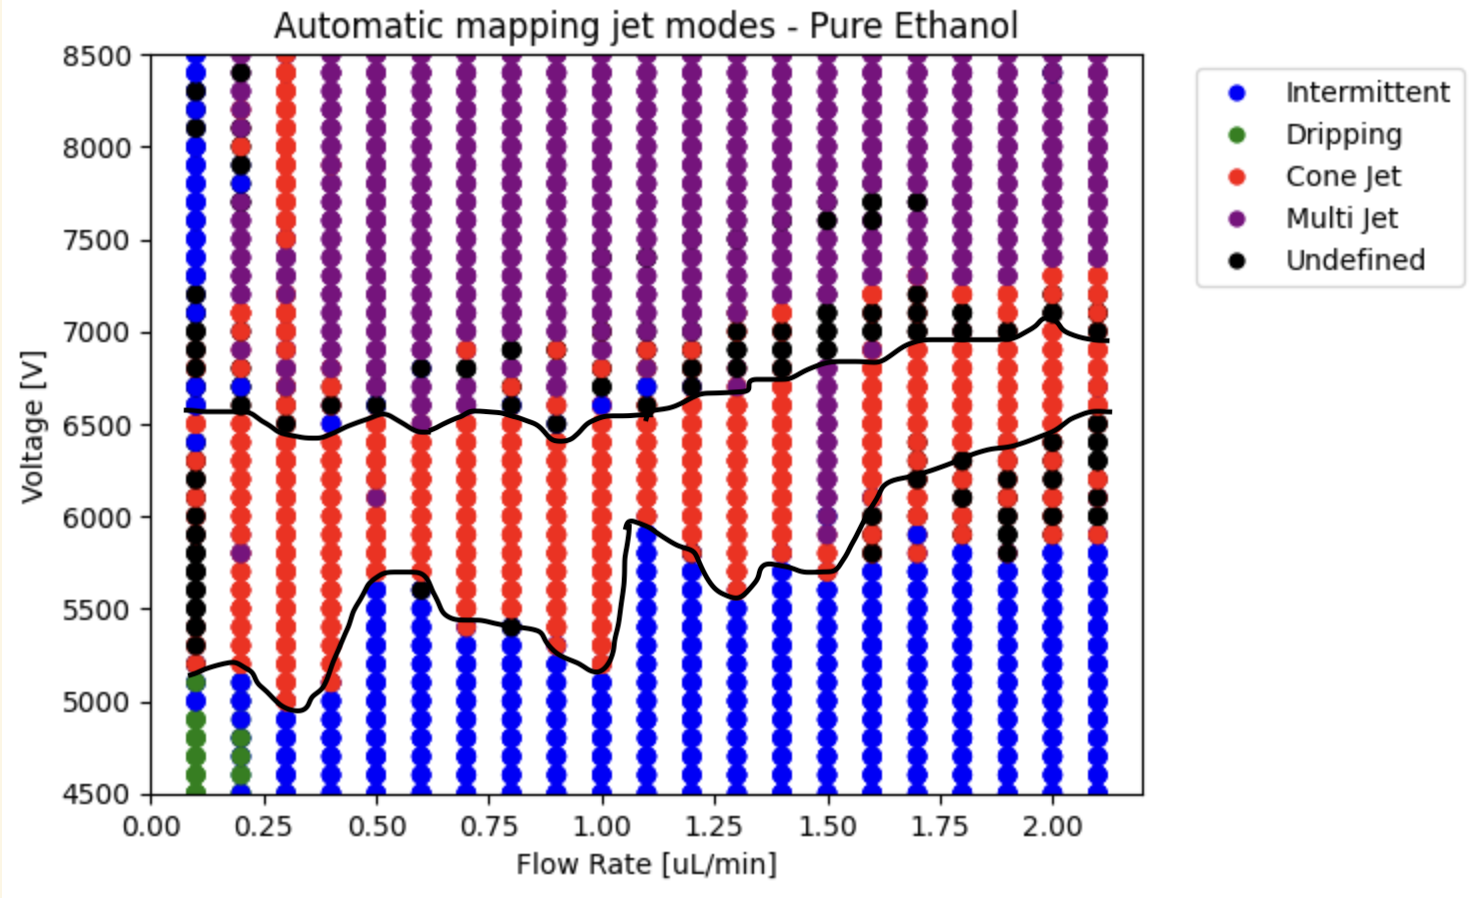
\includegraphics[width=9cm]{Figuras/report4/map7-automatic-line.png}
        \caption{ exp-26-01 automatic classification}
    \end{figure}


\end{multicols}

\subsection{Non-dimensional axis}

\begin{figure}[H]
    \center
    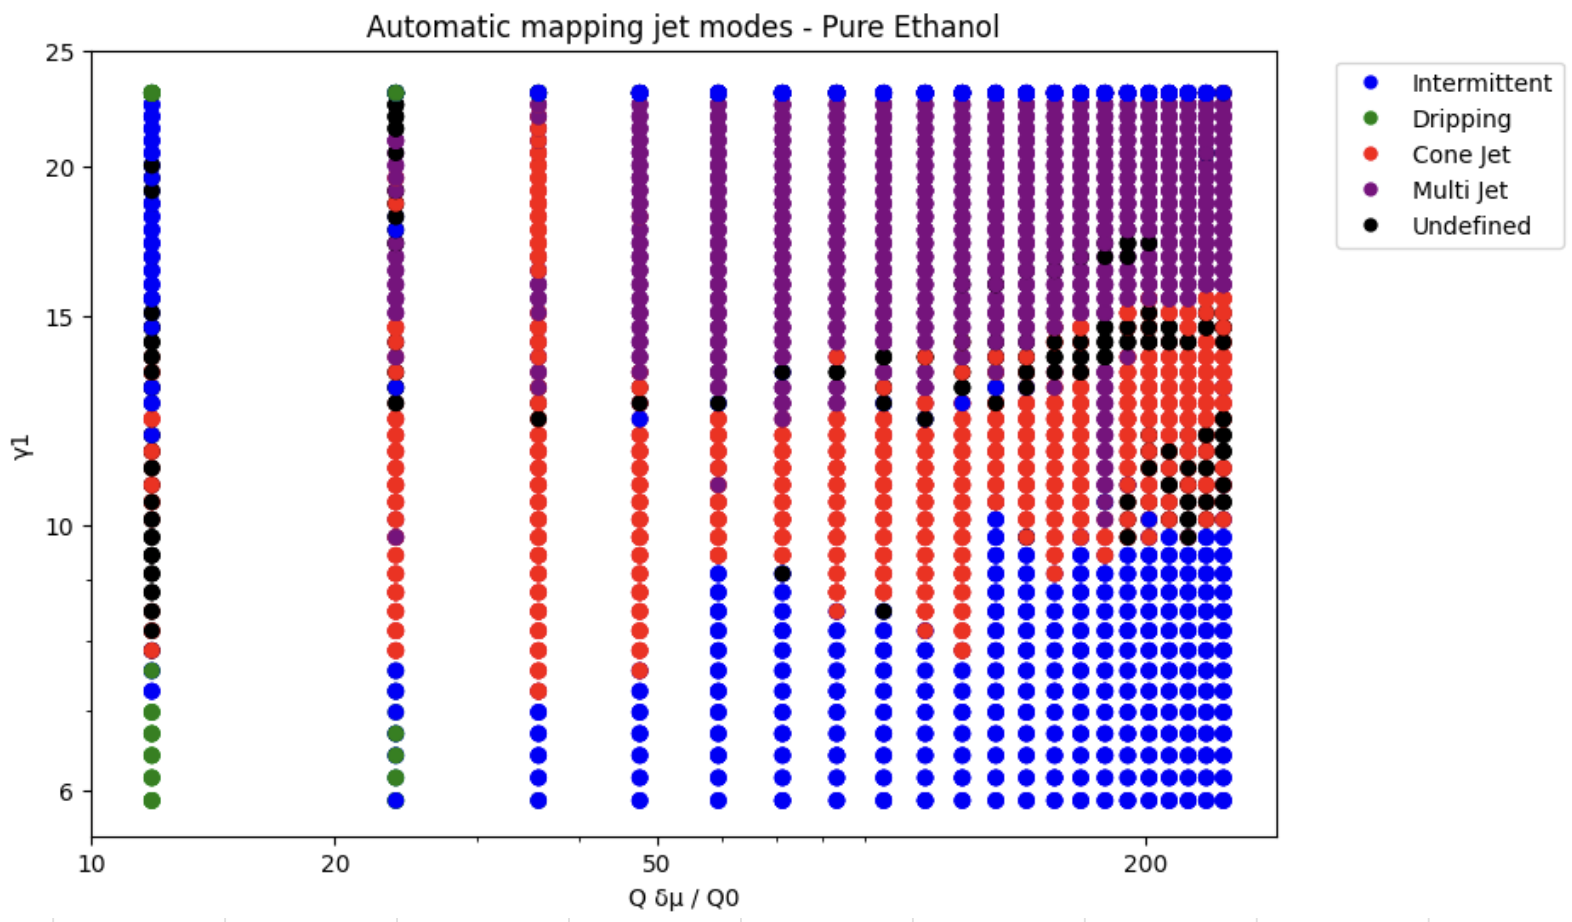
\includegraphics[width=12cm]{Figuras/19:03/non-dimensional-1.png}
    \caption{ exp-26-01-2 (V x Q)}
\end{figure}

\section{Controller}
\label{sec:controller_results}


\subsection{Simple Controller}

\begin{algorithm}
    \caption{simple controller}\label{alg:simple_controller}
    \begin{algorithmic}
    \Function{controller}{$spray\_mode$} 
        
        \If{$spray\_mode$ = $'Intermittent'$ or $spray\_mode$ = $'Dripping'$}
            \State \Call{send\_voltage\_command}{$voltage$ + 100}
        \ElsIf{$spray\_mode$ = $'Multi Jet'$ or $spray\_mode$ = $'Corona'$}
            \State \Call{send\_voltage\_command}{$voltage$ - 100}
        \ElsIf{ $spray\_mode$ = $"Cone Jet"$}
            \Comment{Keep Stable}
        \EndIf

    \Return $spray\_ mode$
    \EndFunction
    \end{algorithmic}
\end{algorithm}

Flowrate perturbation robustness test

\begin{figure}[H]
    \center
    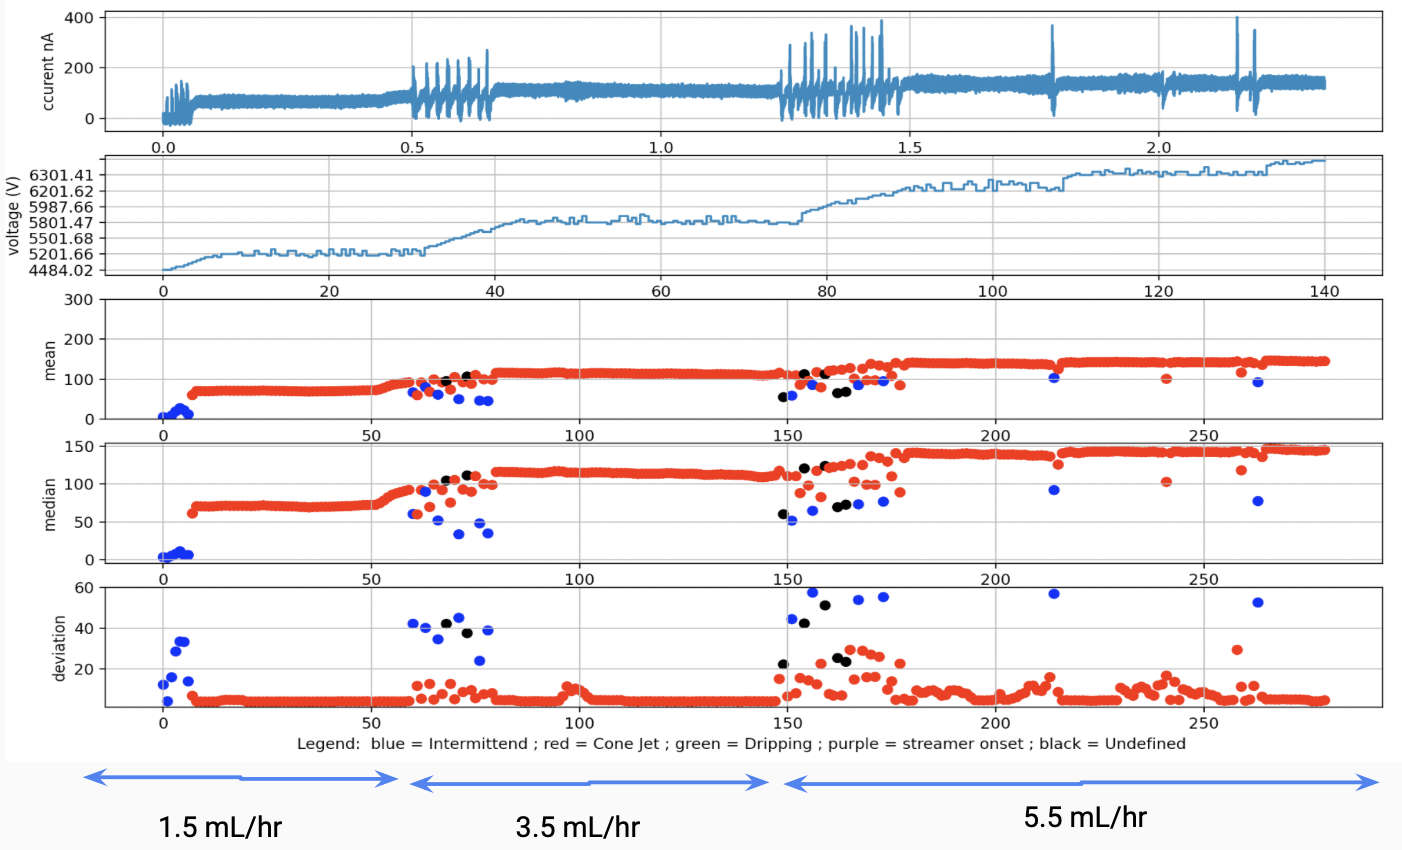
\includegraphics[width=15cm]{Figuras/19:03/control_first_results.png}
    \caption{ exp-26-01-2 (V x Q)}
\end{figure}


\section{Atividades do Projeto}
\label{metodo3}

\section {Requisitos do Sistema}
\label{req}


\clearpage